\subsubsection{Problem Motivation}
\begin{itemize}[--]
	\item Imagine you're an aircraft engine manufacturing, and you measure multiple features $\{x^{(1)},\ldots ,x^{(m)} \}$ off your engines
	\item Lets say given a new engine $x_{test}$, is this aircraft engine anomalous in any way. Should it undergo further testing?
	\item If $p(x_{test}) < \epsilon\to$ flag anomaly
	\item Else $p(x_{test}) \geq\epsilon$ okay
	\item Applications:
	\begin{itemize}[--]
		\item Fraud detection
		\begin{itemize}[--]
			\item $x^{(i)}$ features of user $i$'s activities
			\item Model $p(x)$ from data
			\item Identify unusual users by checking which have $p(x) < \epsilon$
		\end{itemize}

		\item Manufacturing 
		\item Monitoring computers in a ata center
	\end{itemize}
\end{itemize}

\subsubsection{Gaussian Distribution}
\begin{itemize}[--]
	\item Say $x\in\mathbb{R}$. If $x$ is a distributed Gaussian with mean $\mu$, variance $\sigma^2$.
		$$x~\mathcal{N}(\mu, \sigma^2$$
	\item It will look like a bell shaped curve, with peak at $\mu$:
	\begin{center}
		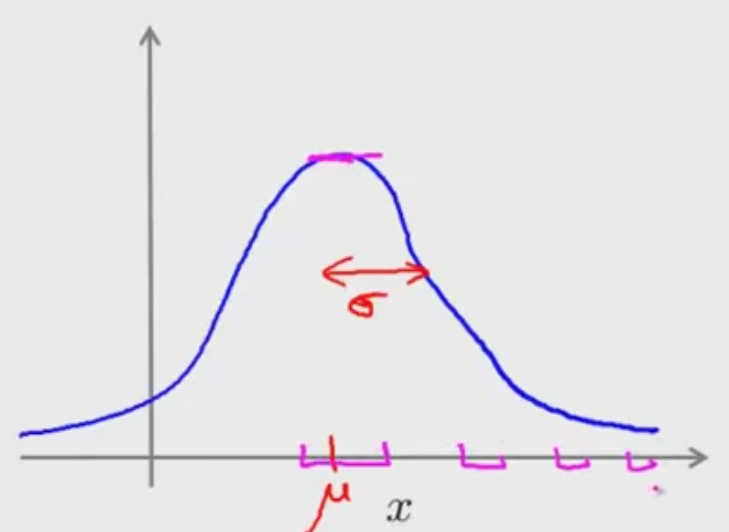
\includegraphics[scale=0.5]{sections/cs229/w12/gaus.png}
	\end{center}
	$$p(x;\mu, \sigma^2)=\frac{1}{\sqrt{2\pi}\sigma} \text{exp}(-\frac{(x-\mu)^2}{2\sigma^2})$$

	\item 
\end{itemize}

\subsubsection{Algorithm}
\begin{itemize}[--]
	\item Density estimation
	\begin{itemize}[--]
		\item Training set $\{ x^{(m)}\}\in\mathbb{R}^n$
			$$p(x)=p(x_1; \mu_1, \sigma_1^2 ) \ldots p(x_n; \mu_n, \sigma_n^2)$$
		\item This corresponds to an independnce assumption (not necessary to use this algorithm)
	\end{itemize}
	\item Algorithm:
	\begin{itemize}[--]
		\item Choose features $x_i$ that you think might be indicative of anomalous examples
		\item Fit parameters $\mu_1, \ldots, \mu_n, \sigma_1^2, \ldots, \sigma_n^2$
			$$\mu_j = \frac{1}{m}\sum_{i=1}^m x_j^{(i)}$$
			$$\sigma^{2}_j = \frac{1}{m}\sum_{i=1}^m (x_j^{(i)} - \mu_j )^2$$
		\item Given new example $x$, compute $p(x)$:
			$$p(x)=\prod_{j=1}^n p(x_j ; \mu_j, \sigma_j^2 )$$
		\item Anomaly if $p(x)< \epsilon$
	\end{itemize}
\end{itemize}

\subsubsection{Developing and Evaluating an Anomaly Detection System}
\begin{itemize}[--]
	\item When developing a learning algorithm (choosing features, etc.), making decisions is much easier if we have a way of evaluating our learning algorithm
	\item Assume we have some labeled data, of anomalous and non-anomalous examples ($y=0$ if normal, $y=1$ if anomalous).
	\item Training set: $x^{(1)},\ldots, x^{(m)}$ (assume normal examples/not anomalous)
	\item Cross validation set: $\{ (x_{cv}^{(m_{cv})}, y_{cv}^{(m_{cv})}\}$
	\item Test set: $\{ x_{test}^{(m_{test})}, y_{test}^{(m_{test})}\}$
	\item Given the aircraft example: 10000 good (normal) engines, 20 flawed engines (anomalous)
	\begin{itemize}[--]
		\item Training set: 6000 good engines ($y=0$)
		\item CV: 2000 good engines, 10 anomalous ($y=1$)
		\item Tset: 2000 good, 10 anomalous
	\end{itemize}

	\item Algorithnm evaluation:
	\begin{itemize}[--]
		\item Fit model $p(x)$ on training set $\{ x^{(m)}\}$
		\item On a cross validation/test example $x$, predict:
			$$y=\begin{cases}
				1 & p(x)< \epsilon \\
				0 & p(x) \geq\epsilon
			\end{cases}$$
		\item Possible evaluation metrics:
		\begin{itemize}[--]
			\item True positives, false positive, false negative, true negative
			\item Precision/Recall
			\item $F_1$ score
		\end{itemize}
		\item Can also use cross validation set to choose parameter $\epsilon$
	\end{itemize}
\end{itemize}

\subsubsection{Anomaly Detection vs. Supervised Learning}
\begin{itemize}[--]
	\item Anomaly Detection
	\begin{itemize}[--]
		\item Very small number of positive examples ($y=1$). (0-20 is common).
		\item Large number of negatives ($y=0$) examples
		\item Many differet ``types'' of anomalies. Hard for any algorithm to learn from positive examples what the anomalies look like; future anomalies may look nothing like any of the anomalous examples we've seen so far
	\end{itemize}

	\item Supervised Learning:
	\begin{itemize}[--]
		\item Large number of positive and negative examples
		\item Enough positive examples for algorithm to get a sense of what positive examples are like, future positive examples likely tob e similar to ones in training set
	\end{itemize}

	\item In anomaly detection, we typically have very small postivie examples, so there's not enough to learn about them
\end{itemize}

\subsubsection{Choosing What Features to Use}
\begin{itemize}[--]
	\item When plotting the probabilities from the anomaly detection we hope to get a gaussian distribution:
	\begin{center}
		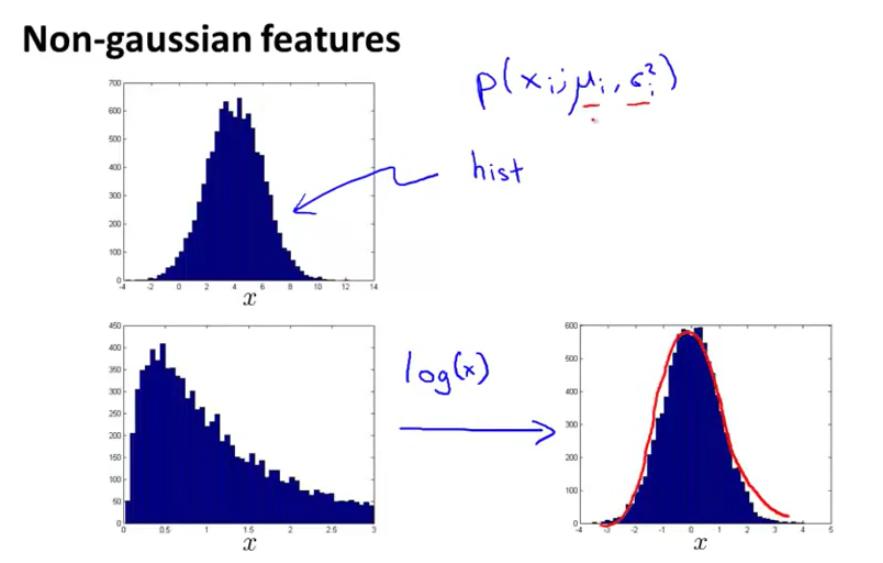
\includegraphics[scale=0.5]{sections/cs229/w12/gausfeat.png}
	\end{center}
	\item However, sometimes we get a skewed distribution, and it's best to attempt to transform (eg. $\log{x_i + c}\to x_i$) this data into a guassian distribution.
	\item Error analysis for anomaly detection
	\begin{itemize}[--]
	 	\item Want $p(x)$ large for normal examples $x$, and small for anomalous examples
	 	\item Most common problem: $p(x)$ is comparable (say, both large) for normal and anomalous examples
	 	\item One way to help pull out the anomaly, is to come up with another feature that makes it easier to distinguish anomalies 
	 \end{itemize}
	 \item Choose features that might take on unusally large or small values in the vent of an anomaly (eg. network traffic, CPU load)
\end{itemize}

\subsubsection{Multivariate Gaussian Distribution}
\begin{itemize}[--]
	\item Lets say we have unlabelled data:
	\begin{center}[--]
		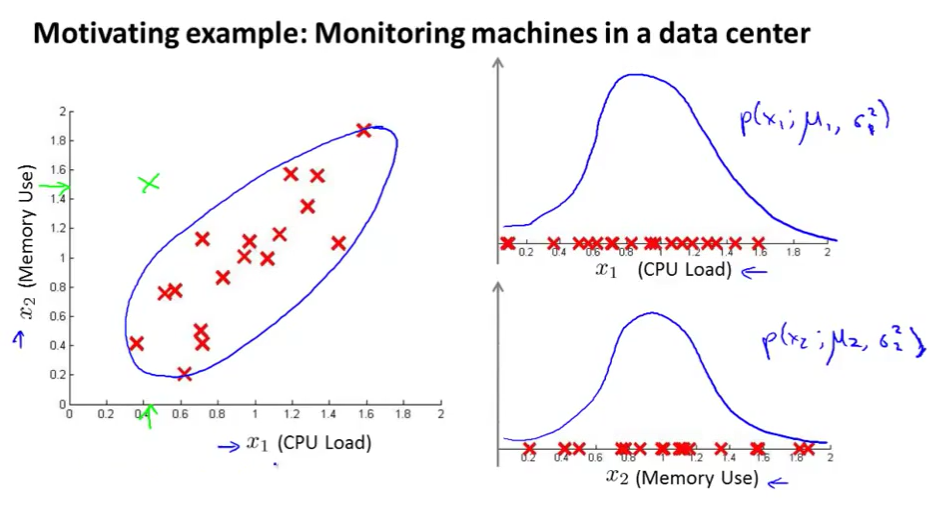
\includegraphics[scale=0.5]{sections/cs229/w12/multi.png}
	\end{center}
	\item Where we have an anomaly (green)
	\item This anomaly, doesn't appear to be an outlier in either 1D plot
	\item This keeps a 	`circular' regions of probability
	\item $x\in\mathbb{R}^{n}$. Don't model $p(x_1),\ldots$ separately. Model $p(x)$ all in one go.
	\item Parameters: $\mu\in\mathbb{R}^n$, $\sigma\in\mathbb{R}^{n\times n}$ (covariance matrix)
		$$p(x;\mu, \sigma)=\frac{1}{(2u\pi)^{n/2} |\sigma |^{0.5}} \text{exp} (-0.5 (x-\mu)^T \sigma^{-1} (x-\mu))$$
	\begin{center}[--]
		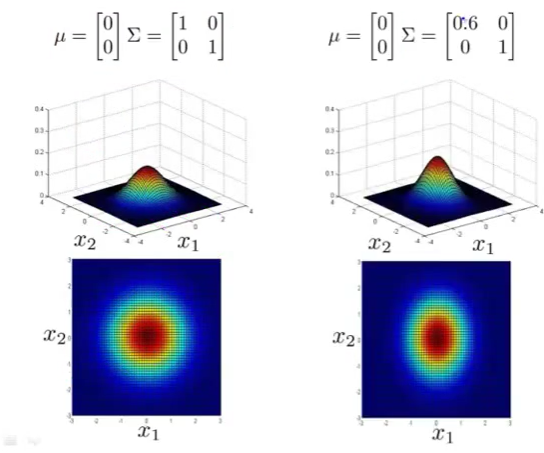
\includegraphics[scale=0.5]{sections/cs229/w12/ex.png}
	\end{center}
	\item As you decrease $\sigma$ you get a smaller steeper curve, in the direction of the col/row you varied
	\item $\mu$ similarly models the point where the curve is centered
	\item You can also model correlactions with the off-diagonal entries
	\begin{center}[--]
		% 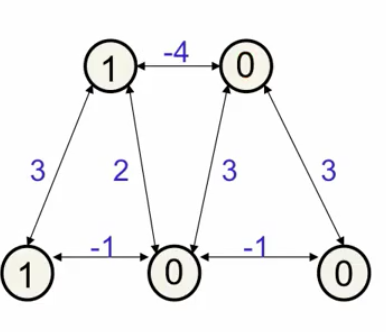
\includegraphics[scale=0.5]{sections/cs229/w12/off.png} TODO: get
	\end{center}
\end{itemize}

\subsubsection{Anomaly Detection using the Multivariate Gaussian Distribution}
\begin{itemize}[--]
	\item Given a training set: $\{ x^{(m)}\}\in\mathbb{R}^n$
		$$\mu = \frac{1}{m}\sum_{i=1}^{m} x^{(i)}$$
		$$\sigma = \frac{1}{m}\sum_{i=1}^{m} (x^{(i)}-\mu ) (x^{(i)}-\mu ) ^T$$
	\item Fit model $p(x)$ by setting these previous parameters	
	\item Given a new example $x$, compute:
		$p(x;\mu, \sigma^2)$
		Flag an anomaly if $p(x)<\epsilon$
	\item The original product model of Gaussian, corresponds to multivariate Gaussian where the distribution is constrained so that the contours are axis aligned
	\item Namely, $\sigma$ has 0's on the off-diagonal entries
	\item When would you use each?
	\item \textbf{Original Model}
	\begin{itemize}[--]
		\item Manually create features to capture anomalies where $x_1, x_2$ takes unusual combinations of values (eg. $x_3=x_1/x_2$)
		\item If you're willing to spend the time creating these features, this model will work fine
		\item Computationally cheaper (alternatively, scalles better to large $n$)
		\item OK even if $m$ (training set size) is small
	\end{itemize}

	\item \textbf{Multivariate Gaussian}
	\begin{itemize}[--]
		\item Automatically captures correlations between features
		\item Computationally more expensive
		\item Must have $m>n$, or else $\sigma$ is non-inverible
		\item $\sigma$ may be non-invertible if there are redundant features ($x_1=x_2, x_3 = x_4 + x_5$), linearly dependent.
	\end{itemize}
\end{itemize}